\documentclass[11pt]{article}

% Preamble

\usepackage[margin=1in]{geometry}
\usepackage{amsfonts, amsmath, amssymb}
\usepackage{fancyhdr, float, graphicx}
\usepackage[utf8]{inputenc} % Required for inputting international characters
\usepackage[T1]{fontenc} % Output font encoding for international characters
\usepackage{fouriernc} % Use the New Century Schoolbook font
\usepackage[nottoc, notlot, notlof]{tocbibind}
\usepackage{listings}
\usepackage{xcolor}
\usepackage{karnaugh-map}

\definecolor{codegreen}{rgb}{0,0.6,0}
\definecolor{codegray}{rgb}{0.5,0.5,0.5}
\definecolor{codepurple}{rgb}{0.58,0,0.82}
\definecolor{backcolour}{rgb}{0.95,0.95,0.92}

\lstdefinestyle{mystyle}{
    backgroundcolor=\color{backcolour},   
    commentstyle=\color{codegreen},
    keywordstyle=\color{magenta},
    numberstyle=\tiny\color{codegray},
    stringstyle=\color{codepurple},
    basicstyle=\ttfamily\footnotesize,
    breakatwhitespace=false,         
    breaklines=true,                 
    captionpos=b,                    
    keepspaces=true,                 
    numbers=left,                    
    numbersep=5pt,                  
    showspaces=false,                
    showstringspaces=false,
    showtabs=false,                  
    tabsize=2
}

\lstset{style=mystyle}

% Header and Footer
\pagestyle{fancy}
\fancyhead{}
\fancyfoot{}
\fancyhead[L]{\textit{\Large{DECA Assignment 2}}}
%\fancyhead[R]{\textit{something}}
\fancyfoot[C]{\thepage}
\renewcommand{\footrulewidth}{1pt}



% Other Doc Editing
% \parindent 0ex
%\renewcommand{\baselinestretch}{1.5}

\begin{document}

\begin{titlepage}
	\centering

	%---------------------------NAMES-------------------------------

	\huge\textsc{
		MIT World Peace University
	}\\

	\vspace{0.75\baselineskip} % space after Uni Name

	\LARGE{
		Digital Electronics and Computer Architecture\\
		Second Year B. Tech, Semester 3
	}

	\vfill % space after Sub Name

	%--------------------------TITLE-------------------------------

	\rule{\textwidth}{1.6pt}\vspace*{-\baselineskip}\vspace*{2pt}
	\rule{\textwidth}{0.6pt}
	\vspace{0.75\baselineskip} % Whitespace above the title



	\huge{\textsc{
			Design and Implementation of Combinational Logic Design using MUX/Decoder ICs.
		}} \\



	\vspace{0.5\baselineskip} % Whitespace below the title
	\rule{\textwidth}{0.6pt}\vspace*{-\baselineskip}\vspace*{2.8pt}
	\rule{\textwidth}{1.6pt}

	\vspace{1\baselineskip} % Whitespace after the title block

	%--------------------------SUBTITLE --------------------------	

	\LARGE\textsc{
		Practical Report
	} % Subtitle or further description
	\vfill

	%--------------------------AUTHOR-------------------------------

	Prepared By
	\vspace{0.5\baselineskip} % Whitespace before the editors

	\Large{
		Krishnaraj Thadesar \\
		Cyber Security and Forensics\\
		Batch A2, PA 34
	}


	\vspace{0.5\baselineskip} % Whitespace below the editor list
	\today

\end{titlepage}


\tableofcontents
\thispagestyle{empty}
\clearpage


\setcounter{page}{1}

\section{Problem Statement}
Design and Implement Combinational Logic Design using MUX/Decoder ICs.

\begin{enumerate}
	\item To Verify the Truth table of multiplexers using IC74153
	\item Design and Implement two variable Functions (SOP and POS) and half adder using IC74LS153
	\item Verify its Truth Table.
	\item Design and implement an 8:1 Multiplexer using two 4:1 Multiplexers for a given function using IC 74LS153.
	      $$
		      Y = f(A, B, C) = \displaystyle\sum_{}^{} m(0, 2, 4, 7)
	      $$
	\item Design and implement 8:1 Multiplexer using One 4:1 Multiplexer, applying reduction method for given function using IC 74LS153
	      $$
		      Y = f(A, B, C) = \displaystyle\sum_{}^{} m(0, 2, 4, 7)
	      $$
\end{enumerate}

\section{ICs Used}

\begin{enumerate}
	\item IC7404 (NOR Gate)
	\item IC7432 (OR Gate)
	\item IC74LS153 (Dual 4: 1 Multiplexer IC)
\end{enumerate}

\section{Platform Used}
Digital Trainer Kit

\section{Theory}

\subsection{What is a Multiplexer}

\begin{itemize}
	\item Multiplexer (MUX) is a network device that allows one or more analog or digital input signals to travel together over the same communications transmission link. The purpose of multiplexing is to combine and transmit signals over a single shared medium in order to optimize efficiency and decrease the total cost of communication.
	\item Essentially, a MUX functions as a multiple-input, single-output switch that allows multiple analog and digital input signals and to be routed through a single output line. At the receiving end, another device called a demultiplexer recovers the original individual signals.
	\item Multiplexers are capable of handling both analog and digital applications. In analog applications, multiplexers are made up of relays and transistor switches, whereas in digital applications, the multiplexers are built from standard logic gates. When the multiplexer is used for digital applications, it is called a digital multiplexer

\end{itemize}

\begin{figure}[H]
	\centering
	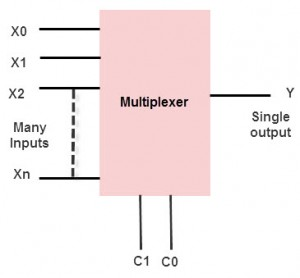
\includegraphics[scale = 0.5]{mux.jpg}
	\caption{Multiplexer Representation}
\end{figure}

\subsubsection{Types}
\begin{enumerate}
	\item 2-1 multiplexer (1 select line)
	\item 4-1 multiplexer (2 select lines)
	\item 8-1 multiplexer(3 select lines)
	\item 16-1 multiplexer (4 select lines)

\end{enumerate}
\subsection{Advantages of a Multiplexer}
\begin{enumerate}
	\item In multiplexer, the usage of a number of wires can be decreased
	\item It reduces the cost as well as the complexity of the circuit
	\item The implementation of a number of combination circuits can be possible by using a multiplexer
	\item Mux doesn't require K-maps and simplification
	\item The multiplexer can make the transmission circuit less complex and economical
	\item The multiplexer ability can be extended to switch audio signals, video signals, etc.
	\item The digital system reliability can be improved using a MUX as it decreases the number of exterior wired connections.
	\item MUX is used to implement several combinational circuits
	\item The logic design can be simplified through MUX
\end{enumerate}
\subsection{Applications of a Multiplexer}

Multiplexers are used in various applications wherein multiple-data need to be transmitted by using a single line.
\begin{enumerate}
	\item Communication Systems \\
	      A communication system has both a communication network and a transmission system. By using a multiplexer, the efficiency of the communication system can be increased by allowing the transmission of data, such as audio and video data from different channels through single lines or cables.

	\item Computer Memory \\Multiplexers are used in computer memory to maintain a huge amount of memory in the computers, and also to reduce the number of copper lines required to connect the memory to other parts of the computer.

	\item Telephone networks:  \\
	      In telephone networks, multiple audio signals are integrated on a single line of transmission with the help of a multiplexer.

	\item Transmission From the computer system of a Sattelite \\
	      The multiplexer is used to transmit the data signals from the computer system of a spacecraft or a satellite to the ground system by using a GSM satellite.

\end{enumerate}
\subsection{Involved Truth Tables}

\subsubsection{OR Gate}

\begin{table}[H]
	\begin{tabular}{|c|c|c|}
		\hline
		{\color[HTML]{000000} \textbf{A}} & {\color[HTML]{000000} \textbf{B}} & {\color[HTML]{000000} \textbf{Q}} \\ \hline
		{\color[HTML]{330001} \textit{0}} & {\color[HTML]{330001} \textit{0}} & {\color[HTML]{F56B00} \textit{0}} \\ \hline
		{\color[HTML]{330001} \textit{0}} & {\color[HTML]{330001} \textit{1}} & {\color[HTML]{F56B00} \textit{1}} \\ \hline
		{\color[HTML]{330001} \textit{1}} & {\color[HTML]{330001} \textit{0}} & {\color[HTML]{F56B00} \textit{1}} \\ \hline
		{\color[HTML]{330001} \textit{1}} & {\color[HTML]{330001} \textit{1}} & {\color[HTML]{F56B00} \textit{1}} \\ \hline
	\end{tabular}
\end{table}
\subsubsection{NOT Gate}

\begin{table}[H]
	\begin{tabular}{|c|c|}
		\hline
		{\color[HTML]{000000} \textbf{A}} & {\color[HTML]{000000} \textbf{Q}} \\ \hline
		{\color[HTML]{000000} 0}          & {\color[HTML]{F56B00} 1}          \\ \hline
		{\color[HTML]{000000} 1}          & {\color[HTML]{F56B00} 0}          \\ \hline
	\end{tabular}
\end{table}
\subsubsection{Truth Table of Half Adder}

\begin{table}[H]
	\begin{tabular}{|c|c|c|c|}
		\hline
		{\color[HTML]{000000} \textbf{A}} & {\color[HTML]{000000} \textbf{B}} & {\color[HTML]{000000} \textbf{Sum}} & {\color[HTML]{000000} \textbf{Carry}} \\ \hline
		{\color[HTML]{000000} 0}          & {\color[HTML]{000000} 0}          & {\color[HTML]{CE6301} 0}            & {\color[HTML]{CE6301} 0}              \\ \hline
		{\color[HTML]{000000} 0}          & {\color[HTML]{000000} 1}          & {\color[HTML]{CE6301} 1}            & {\color[HTML]{CE6301} 0}              \\ \hline
		{\color[HTML]{000000} 1}          & {\color[HTML]{000000} 0}          & {\color[HTML]{CE6301} 1}            & {\color[HTML]{CE6301} 0}              \\ \hline
		{\color[HTML]{000000} 1}          & {\color[HTML]{000000} 1}          & {\color[HTML]{CE6301} 0}            & {\color[HTML]{CE6301} 1}              \\ \hline
	\end{tabular}
\end{table}
\subsubsection{Truth Table of a Full Adder}

\begin{table}[H]
	\begin{tabular}{|c|c|c|c|c|}
		\hline
		{\color[HTML]{000000} \textbf{A}} & {\color[HTML]{000000} \textbf{B}} & {\color[HTML]{000000} \textbf{Cin}} & {\color[HTML]{000000} \textbf{Sum}} & {\color[HTML]{000000} \textbf{Cout}} \\ \hline
		{\color[HTML]{000000} 0}          & {\color[HTML]{000000} 0}          & {\color[HTML]{000000} 0}            & {\color[HTML]{F56B00} 0}            & {\color[HTML]{F56B00} 0}             \\ \hline
		{\color[HTML]{000000} 0}          & {\color[HTML]{000000} 0}          & {\color[HTML]{000000} 1}            & {\color[HTML]{F56B00} 1}            & {\color[HTML]{F56B00} 0}             \\ \hline
		{\color[HTML]{000000} 0}          & {\color[HTML]{000000} 1}          & {\color[HTML]{000000} 0}            & {\color[HTML]{F56B00} 1}            & {\color[HTML]{F56B00} 0}             \\ \hline
		{\color[HTML]{000000} 0}          & {\color[HTML]{000000} 1}          & {\color[HTML]{000000} 1}            & {\color[HTML]{F56B00} 0}            & {\color[HTML]{F56B00} 1}             \\ \hline
		{\color[HTML]{000000} 1}          & {\color[HTML]{000000} 0}          & {\color[HTML]{000000} 0}            & {\color[HTML]{F56B00} 1}            & {\color[HTML]{F56B00} 0}             \\ \hline
		{\color[HTML]{000000} 1}          & {\color[HTML]{000000} 0}          & {\color[HTML]{000000} 1}            & {\color[HTML]{F56B00} 0}            & {\color[HTML]{F56B00} 1}             \\ \hline
		{\color[HTML]{000000} 1}          & {\color[HTML]{000000} 1}          & {\color[HTML]{000000} 0}            & {\color[HTML]{F56B00} 0}            & {\color[HTML]{F56B00} 1}             \\ \hline
		{\color[HTML]{000000} 1}          & {\color[HTML]{000000} 1}          & {\color[HTML]{000000} 1}            & {\color[HTML]{F56B00} 1}            & {\color[HTML]{F56B00} 1}             \\ \hline
	\end{tabular}
\end{table}
\subsubsection{Function Table of the IC74LS153}
\begin{figure}[H]
	\centering
	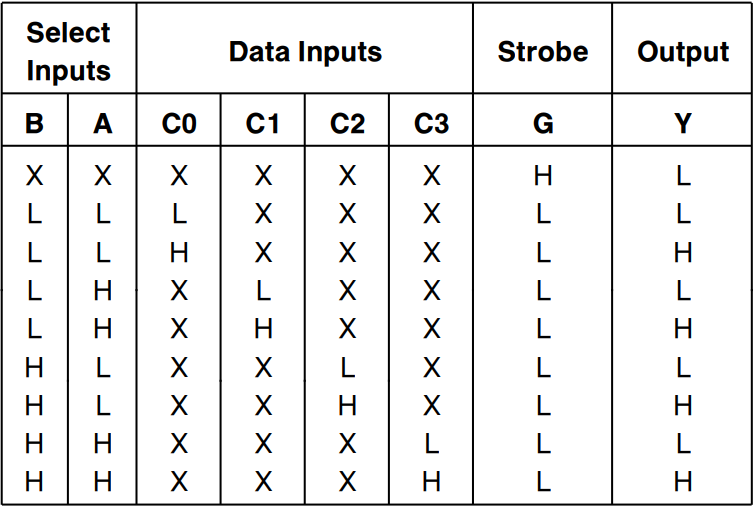
\includegraphics[scale = 0.5]{function_table.png}
	\caption{Function Table for IC 74LS153}
\end{figure}
\subsection{Symbols in the Pin Diagram of IC74LS153}
\begin{table}[H]
	\begin{tabular}{|l|l|l|}
		\hline
		\multicolumn{1}{|c|}{\textbf{Pin}} & \multicolumn{1}{c|}{\textbf{Symbol}} & \multicolumn{1}{c|}{\textbf{Description}} \\ \hline
		1                                  & 1E                                   & enable input 1                            \\ \hline
		2                                  & S1                                   & common data select input                  \\ \hline
		3                                  & 1I3                                  & data input from source 1                  \\ \hline
		4                                  & 1I2                                  & data input from source 1                  \\ \hline
		5                                  & 1I1                                  & data input from source 1                  \\ \hline
		6                                  & 1I0                                  & data input from source 1                  \\ \hline
		7                                  & 1Y                                   & multiplexer output from source 1          \\ \hline
		8                                  & GND                                  & ground                                    \\ \hline
		9                                  & 2Y                                   & multiplexer output from source 2          \\ \hline
		10                                 & 2I0                                  & data input from source 2                  \\ \hline
		11                                 & 2I1                                  & data input from source 2                  \\ \hline
		12                                 & 2I2                                  & data input from source 2                  \\ \hline
		13                                 & 2I3                                  & data input from source 2                  \\ \hline
		14                                 & S0                                   & common data select input                  \\ \hline
		15                                 & 2E                                   & enable input 2                            \\ \hline
		16                                 & Vcc                                  & supply voltage                            \\ \hline
	\end{tabular}
\end{table}
\pagebreak
\subsubsection{Given SOP Function for 4 : 1 Implementation}
$$
	Y = f(A, B, C) = \displaystyle\sum_{}^{} m(0, 2)
$$

\begin{table}[H]
	\begin{tabular}{|l|l|l|l|}
		\hline
		\textbf{Inputs} & \textbf{A} & \textbf{B} & \textbf{Y} \\ \hline
		I0              & 0          & 0          & 1          \\ \hline
		I1              & 0          & 1          & 0          \\ \hline
		I2              & 1          & 0          & 1          \\ \hline
		I3              & 1          & 1          & 0          \\ \hline
	\end{tabular}
\end{table}
\subsubsection{Given POS Function for 4 : 1 Implementation}
$$
	Y = f(A, B, C) = \displaystyle\Pi M(1, 2)
$$

\begin{table}[H]
	\begin{tabular}{|l|l|l|l|}
		\hline
		\textbf{Inputs} & \textbf{B} & \textbf{A} & \textbf{Y} \\ \hline
		I0              & 0          & 0          & 1          \\ \hline
		I1              & 0          & 1          & 0          \\ \hline
		I2              & 1          & 0          & 0          \\ \hline
		I3              & 1          & 1          & 1          \\ \hline
	\end{tabular}
\end{table}
\subsection{Given SOP Function for 8 : 1 Implementation }
$$
	Y = f(A, B, C) = \displaystyle\sum_{}^{} m(0, 2, 4, 7)
$$

\begin{table}[H]
	\begin{tabular}{|l|l|l|l|l|}
		\hline
		\textbf{Decimal} & \textbf{C} & \textbf{B} & \textbf{A} & \textbf{Output} \\ \hline
		0                & 0          & 0          & 0          & 1               \\ \hline
		1                & 0          & 0          & 1          & 0               \\ \hline
		2                & 0          & 1          & 0          & 1               \\ \hline
		3                & 0          & 1          & 1          & 0               \\ \hline
		4                & 1          & 0          & 0          & 1               \\ \hline
		5                & 1          & 0          & 1          & 0               \\ \hline
		6                & 1          & 1          & 0          & 0               \\ \hline
		7                & 1          & 1          & 1          & 1               \\ \hline
	\end{tabular}
\end{table}

\section{Pin Diagrams of ICs Used}

\subsection{Pin Diagram of IC74LS153}
\begin{figure}[H]
	\centering
	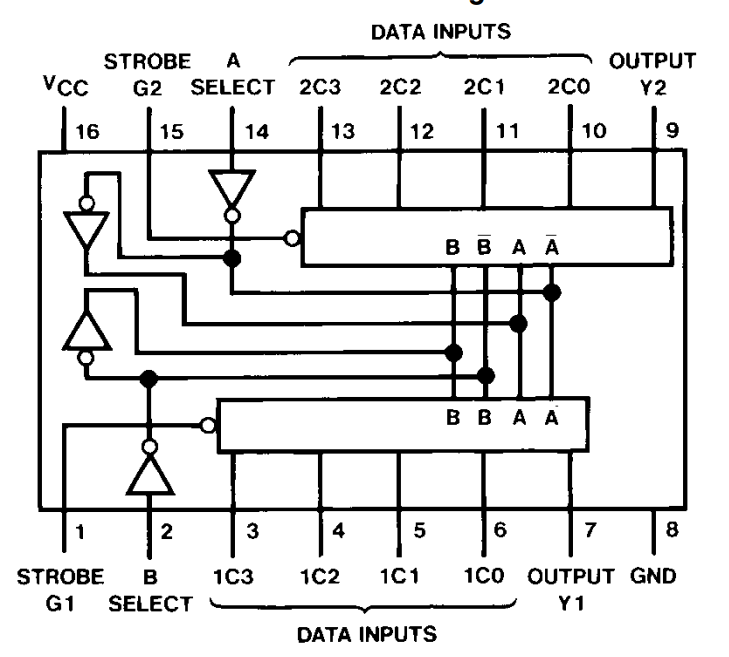
\includegraphics[scale = 0.5]{pin_diagram_74153.png}
	\caption{Pin Diagram for IC 74LS153}
\end{figure}
\subsection{Pin Diagram of IC7432}
\begin{figure}[H]
	\centering
	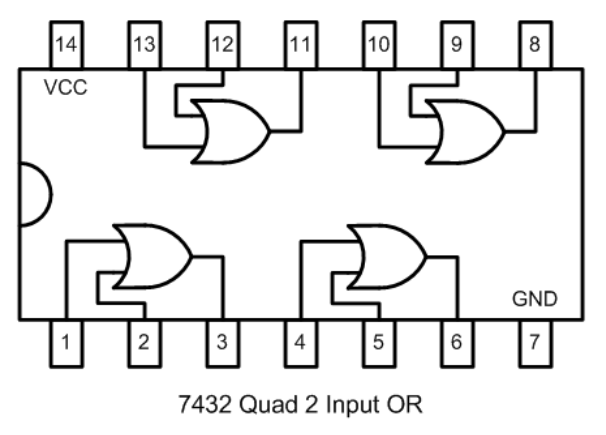
\includegraphics[scale = 0.6]{7432.png}
	\caption{Pin Diagram for IC 7432}
\end{figure}
\subsection{Pin Diagram of IC7404}
\begin{figure}[H]
	\centering
	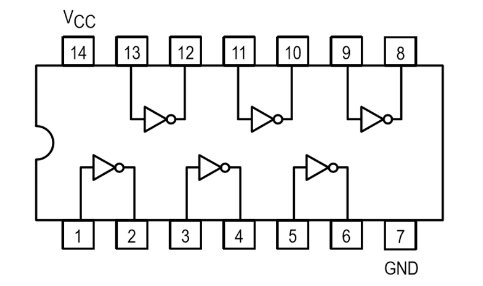
\includegraphics[scale = 0.8]{7404.png}
	\caption{Pin Diagram for IC 7404}
\end{figure}

\section{Design and Implementation}

\subsection{Logical Design for Verification of Truth Table of IC74LS153}
\begin{figure}[H]
	\centering
	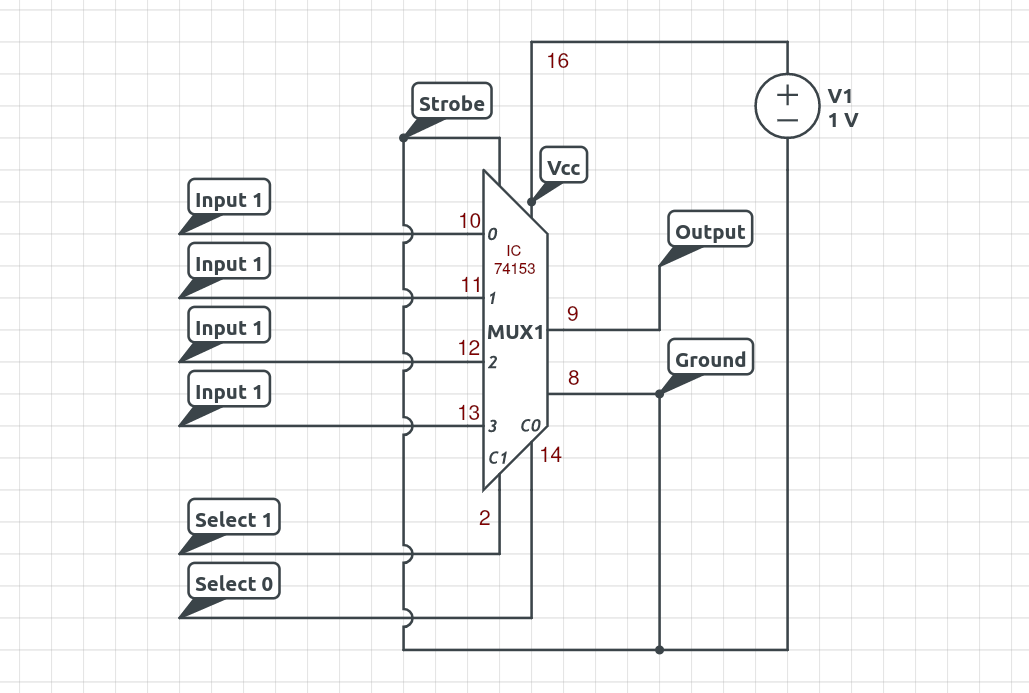
\includegraphics[scale = 0.55]{Truth Table.png}
	\caption{Truth Table for IC 74153}
\end{figure}
\subsection{Logical Design of SOP on 4: 1 Multiplexer using IC74LS153}
$$
	Y = f(A, B, C) = \displaystyle\sum_{}^{} m(0, 2)
$$

\begin{figure}[H]
	\centering
	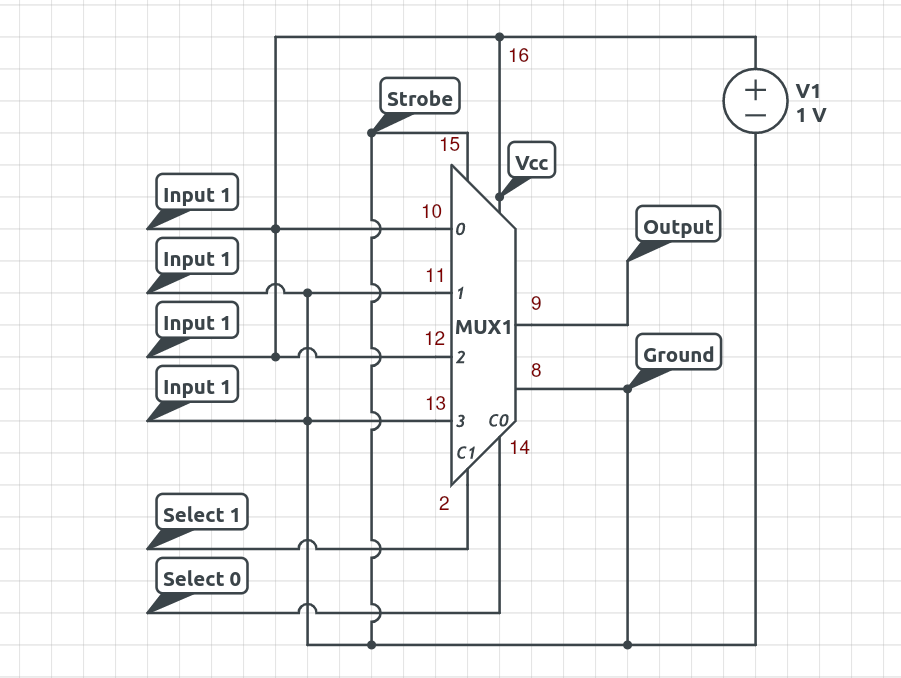
\includegraphics[scale = 0.45]{sop.png}
	\caption{Diagram for Implementation of SOP}
\end{figure}
\subsection{Logical Design of POS on 4: 1 Multiplexer using IC74LS153}
$$
	Y = f(A, B, C) = \displaystyle\Pi M(1, 2)
$$
\begin{figure}[H]
	\centering
	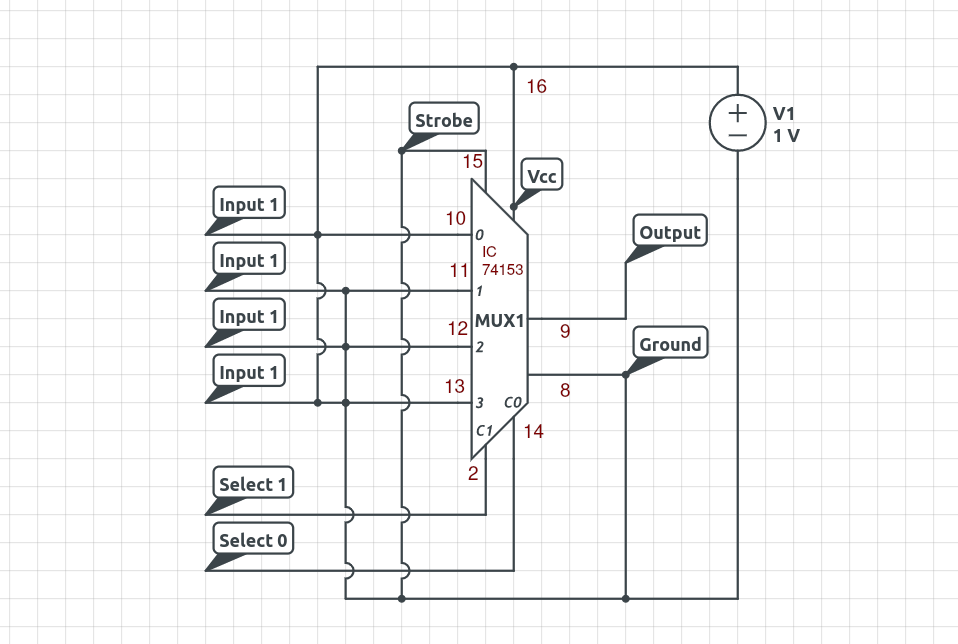
\includegraphics[scale = 0.5]{pos.png}
	\caption{Diagram for Implementation of POS}
\end{figure}
\subsection{Logical Design of Half Adder using IC74LS153}
\begin{figure}[H]
	\centering
	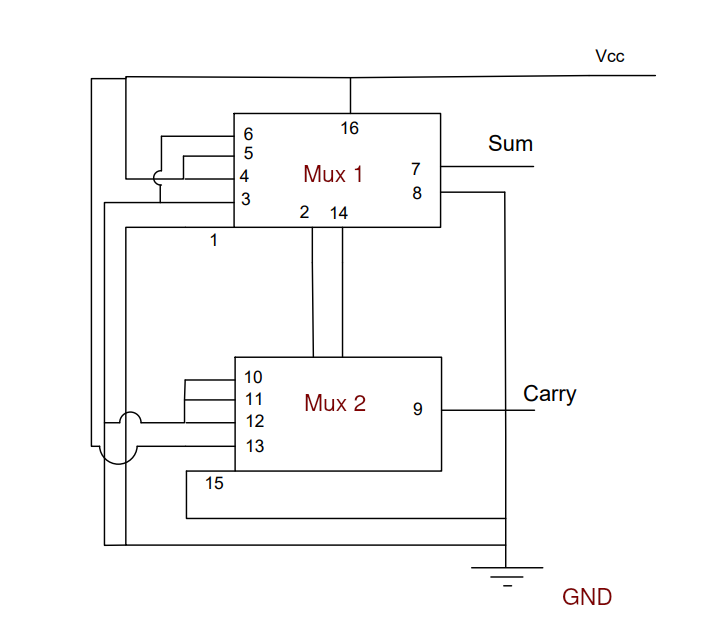
\includegraphics[scale = 0.8]{half adder.png}
	\caption{Half Adder Implementation using 2 4:1 Mux}
\end{figure}
\subsection{Logical Design of Full Adder using IC74LS153}
\vfill
\begin{figure}[H]
	\centering
	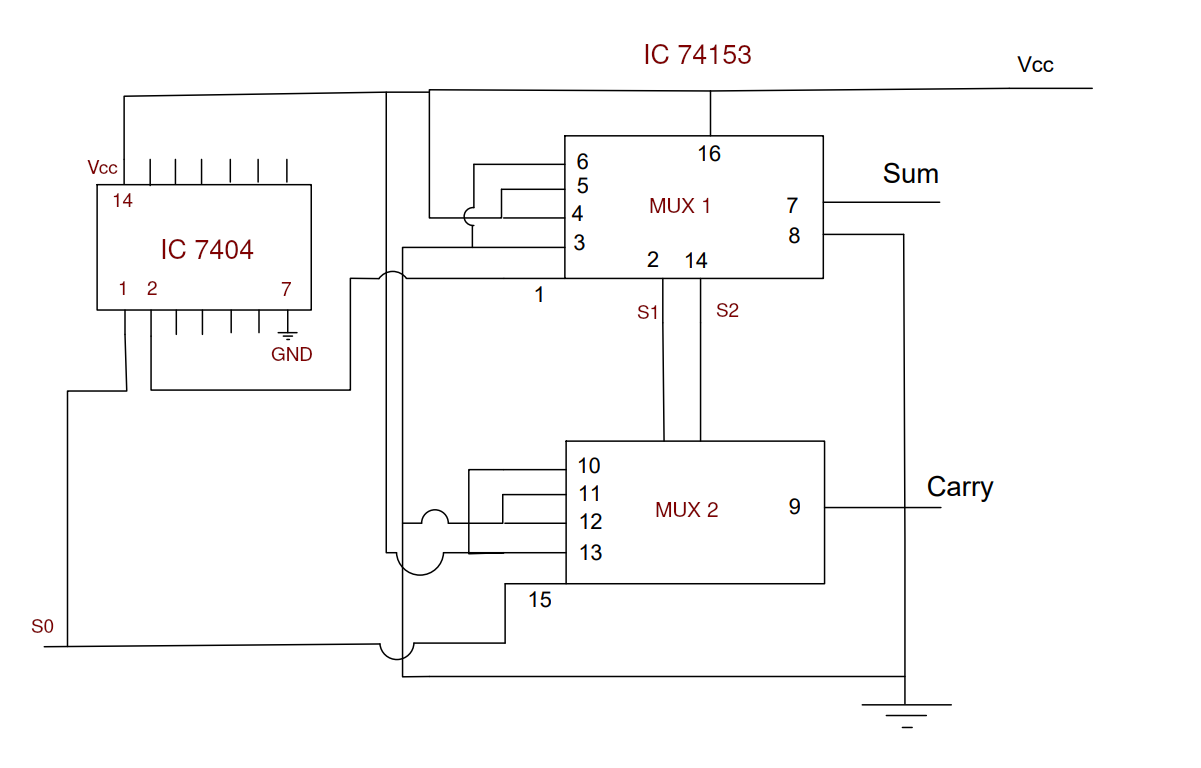
\includegraphics[scale = 0.6]{full adder.png}
	\caption{Full Adder Implementation using 2 4:1 Mux}
\end{figure}

\vfill
\pagebreak
\subsection{Logical Design for Implementing 8 : 1 Multiplexer using 2 4: 1 Multiplexers in IC74LS153 for Given SOP Function}
$$
	Y = f(A, B, C) = \displaystyle\sum_{}^{} m(0, 2, 4, 7)
$$
\vfill
\begin{figure}[H]
	\centering
	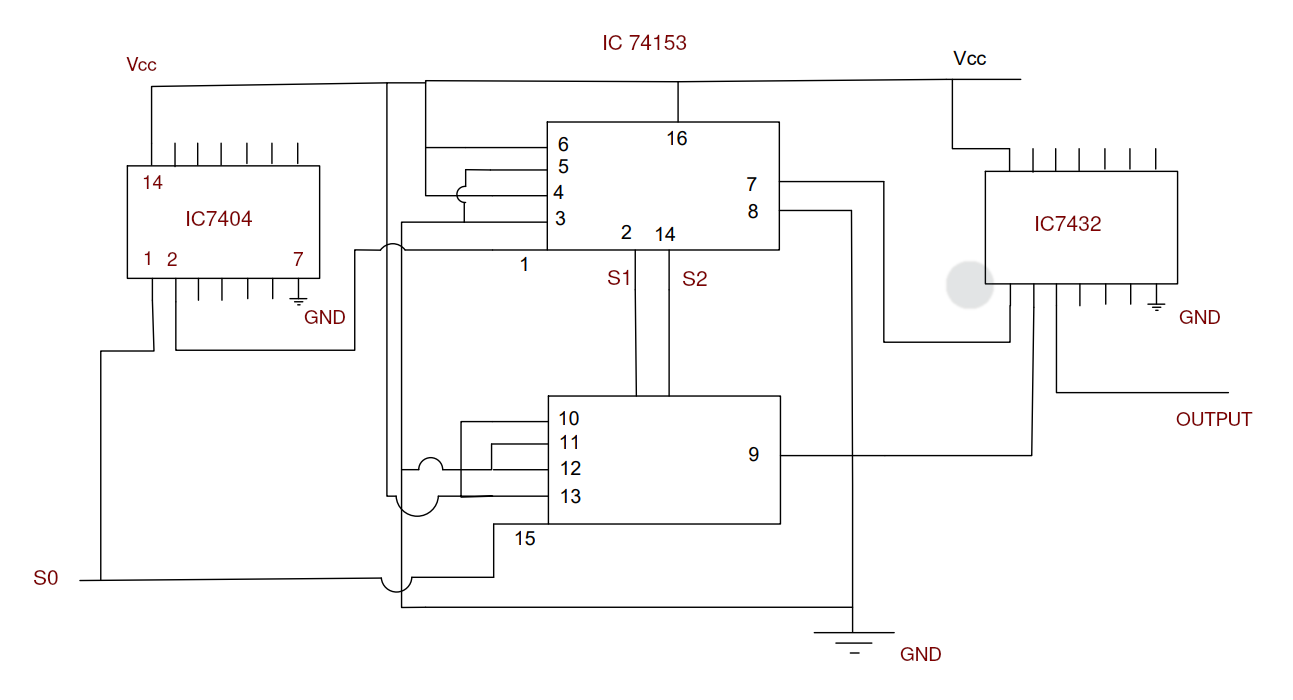
\includegraphics[scale = 0.5]{function implementation using 2 mux.png}
	\caption{Given SOP Function Implementation 2 4:1 Mux}
\end{figure}
\vfill
\pagebreak
\subsection{Logical Design for Implementing 8 : 1 Multiplexer using only 1 4: 1 Multiplexers in IC74LS153 for Given SOP Function using Reduction Method}
$$
	Y = f(A, B, C) = \displaystyle\sum_{}^{} m(0, 2, 4, 7)
$$

\textbf{Reduction Method} \\


\begin{karnaugh-map}[4][2][1][$I_2I_3$][$I_0I_1$][$A$]
\manualterms{1, 0, 0, 1, 1, 0, 1, 0}
% \autoterms[0]
\implicant{0}{4}
\implicant{3}{3}
\implicant{6}{6}
\end{karnaugh-map}

\begin{eqnarray}
	I_0 = V_{cc}\\
	I_1 = GND\\
	I_2 = \overline{A}\\
	I_3 = A
\end{eqnarray}

\begin{figure}[H]
	\centering
	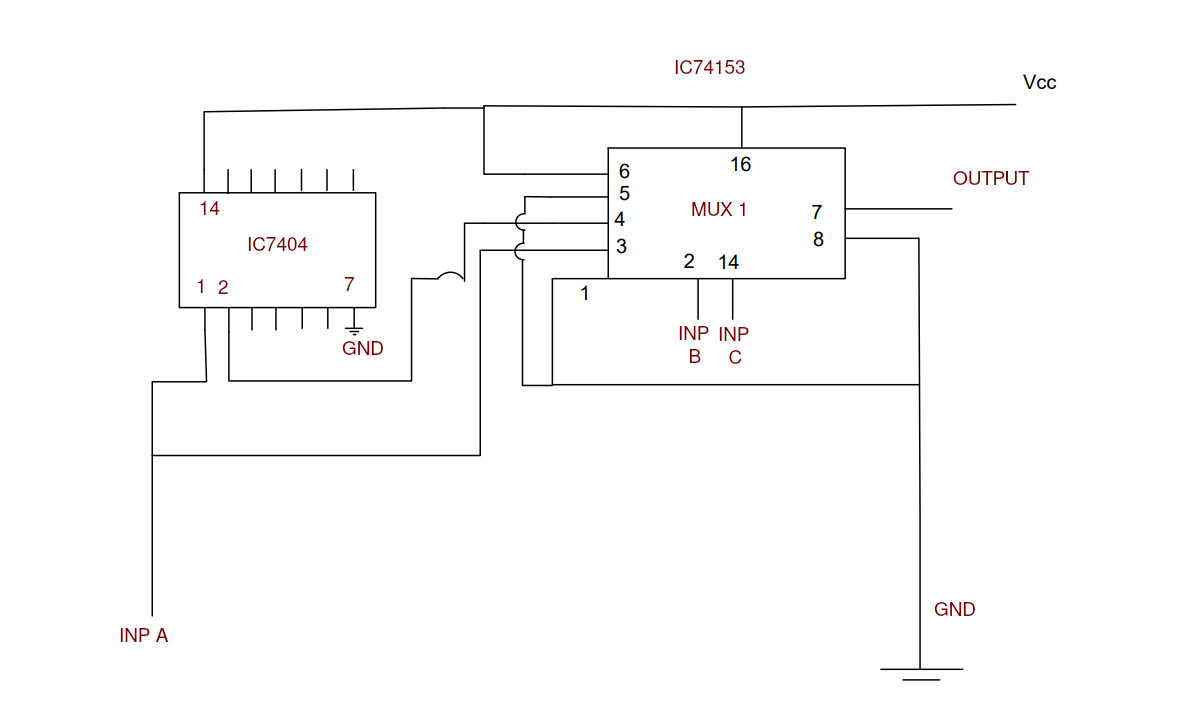
\includegraphics[scale = 0.5]{function implementation using 1 mux.png}
	\caption{Given SOP Function Implementation 1 4:1 Mux}
\end{figure}

\section{Procedure}

\begin{enumerate}
	\item Design Combinational logic circuit as per given problem statement.
	\item Connect the IC 74153 and other basic logic gate ICs as per diagram.
	\item Give Vcc supply and ground connection to each IC.
	\item Give various combinations to select lines.
	\item Observe the output and verify the truth table.
	\item Switch off the power supply of the trainer kit.
\end{enumerate}

\section{Conclusion}
We have learnt the application, usage and implementation of Multiplexers. SOP and POS Implementations on MUX were also understood. The Functionalities of Half Adder and Full adder were learnt in detail, and we also learnt how to apply basic logic gates in a different circuit according to its requirements.

\pagebreak
\section{FAQs}

\begin{enumerate}
	\item \textbf{ What is the use of Strobe in a Multiplexer?}
	      Strobe is the enable pin in MUX. It is the pin that enables the functioning of the MUX. Depending on it being Active Low or Active High, If we pass deactivating signal to strobe, none of the inputs are selected in the MUX. Each mux has a Strobe.
	\item \textbf{Design and Implement a Full Adder using a Multiplexer}
	      Implementation, Diagram and Truth Table are given above.
\end{enumerate}

\end{document}